\documentclass[a4paper]{article}
\usepackage[utf8]{inputenc}
\usepackage{amsmath,float,amsfonts,amssymb,amsthm}
\usepackage{graphicx}
\usepackage{parskip}

% \begin{figure}[H!]
%     
\includegraphics[width=0.25\linewidth]{BUET_LOGO.png}
% \end{figure}

\title{{\centering 
{\textbf{BANGLADESH UNIVERSITY OF ENGINEERING AND TECHNOLOGY}} \\
{\small \text{DEPARTMENT OF COMPUTER SCIENCE AND ENGINEERING}}\\
\vspace{1cm}
{ \begin{Large}{CSE 306 (Computer Architecture Sessional)}\end{Large}}\\[36pt]
% \begin{center}
% \begin{table}[H]
% \centering
%     \begin{tabular}{c}
%         \hline
%         \\
%         \begin{Huge}
%                 \textbf{4-bit MIPS Design}
%         \end{Huge}
%         \\
%         \\
%         \begin{Huge}
%             \textbf{Simulation and Implementation}
%         \end{Huge}
%         \\
%         \\
%         \hline
%         \\
%     \end{tabular}
% \end{table}
% \end{center}

\begin{figure}[H]
    \centering
    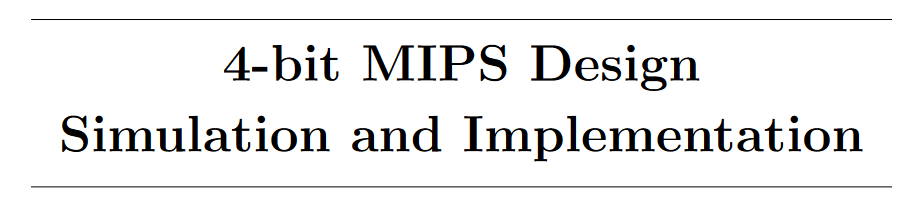
\includegraphics[width=1\linewidth]{image.png}
\end{figure}

\vspace{0.8cm}
\textbf{Subsection: A2}\\
    {\texttt {Group 6}}
    \vspace{0.8cm}
}}
\author{
  Gourab Biswas\\
  \texttt{2005034}
  \and
  Md. As-Aid Rahman\\
  \texttt{2005039}
  \and
  Md. Farhad Al Amin Dipto\\
  \texttt{2005042}
  \and
  Mahamudul Hasan Fahim\\
  \texttt{2005043}
  \and
  Sabbir Alam Saad\\
  \texttt{2005059}
  \vspace{1.2cm}
}
\date{\today}

\begin{document}
\pagenumbering{gobble}
\maketitle
\vspace{4cm}
\thispagestyle{empty}
\vspace{4cm}
\tableofcontents
\vspace{2cm}
\newpage
\listoffigures
\vspace{2cm}
\listoftables

\newpage
\clearpage
\pagenumbering{arabic}

\section{Introduction}
MIPS is a RISC (Reduced Instruction Set Computer) ISA (Instruction Set Architecture).
Instructions of MIPS are fixed, thus ensuring regularity.
Here is an example of add instruction.

\begin{table}[h!]
    \centering
    \begin{tabular}{|c|c|c|}
    \hline
        Operation & Instruction & Action \\
    \hline
        Addition & add \$t2, \$t1, \$t3 & \$t2 = \$t1 + \$t3 \\
    \hline
    \end{tabular}
\end{table}

Here \$t1, \$t2, \$t3 are registers that hold values. To evaluate an expression $ x = a + b – c $, we would do the following:

add \$t0, \$t1, \$t2 [ $x = a + b$ ] \\
add \$t0, \$t0, \$t3 [ $x = x + c$ or $x = a + b + c$ ]

According to MIPS instruction rules, arithmetic operations can only take registers as arguments, size of a register is 32 bits and there are 32 registers in total.\\
A datapath is built with registers, ALUs, MUXs, memories and controls elements that can process data and addresses in the CPU. MIPS instructions are fed through a datapath to perform various instructions like addition, load/store, branching or jump.

\section{Problem Specification}
\subsection{Instruction Set}
We have been assigned to implement a modified and reduced
version of the MIPS instruction set. Our implementation will feature an 8-bit address bus and a 4-bit data bus, as well as a 4-bit ALU, hence the name 4-bit MIPS. As part of our design, we need to include several temporary registers, including \$zero, \$t0, \$t1, \$t2, \$t3, and \$t4.\\

\begin{center}
    \textbf{MIPS INSTRUCTION FORMAT}
\end{center}
\begin{figure}[H]
    \centering
    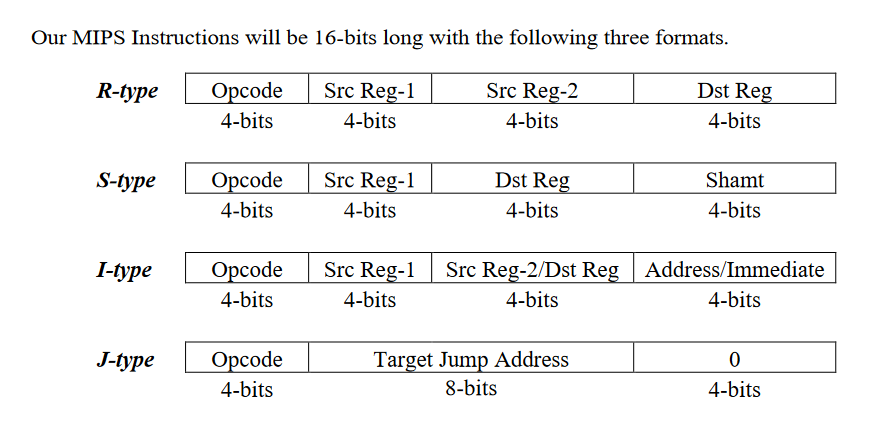
\includegraphics[width=1\linewidth]{InstructionFormat.pdf.png}
    \label{fig:enter-label}
\end{figure}

Instruction set for our MIPS is given below.
\begin{table}[H]
    \centering
    \caption{INSTRUCTION SET DESCRIPTION}
    \vspace{0.5cm}
    \begin{tabular}{|c|c|c|c|}
    \hline
    Instruction ID & Category & Type & Instruction\\
    \hline
    A & Arithmetic & R & add\\
    \hline
    B & Arithmetic & I & addi\\
    \hline
    C & Arithmetic & R & sub\\
    \hline
    D & Arithmetic & I & subi\\
    \hline
    E & Logic & R & and\\
    \hline
    F & Logic & I & andi\\
    \hline
    G & Logic & R & or\\
    \hline
    H & Logic & I & ori\\
    \hline
    I & Logic & S & sll\\
    \hline
    J & Logic & S & srl\\
    \hline
    K & Logic & R & nor\\
    \hline
    L & Memory & I & sw\\
    \hline
    M & Memory & I & lw\\
    \hline
    N & Control-conditional & I & beq\\
    \hline
    O & Control-conditional & I & bneq\\
    \hline
    P & Control-unconditional & J & j \\
    \hline
    \end{tabular}
\end{table}

Opcodes of the instructions are of 4 bits, so between 0 and 15. We’re given the Instruction assignment \textbf{AHLOGBFNMJDPECKI}. So, our opcodes will point to corresponding operations as described below:


\begin{table}[H]
    \centering
    \begin{tabular}{|c|c|}
    \hline
         Opcode & Operation \\
         \hline
            0000 & add\\
            \hline
            0001 & ori\\
            \hline
            0010 & sw\\
            \hline
            0011 & bneq\\
            \hline
            0100 & or\\
            \hline
            0101 & addi\\
            \hline
            0110 & andi\\
            \hline
            0111 & beq\\
            \hline
            1000 & lw\\
            \hline
            1001 & srl\\
            \hline
            1010 & subi\\
            \hline
            1011 & j\\
            \hline
            1100 & and\\
            \hline
            1101 & sub\\
            \hline
            1110 & nor\\
            \hline
            1111 & sll\\
            \hline
    \end{tabular}
\end{table}

\section{Complete Block diagram of a 4-bit MIPS processor}

\begin{figure}[H]
    \centering
    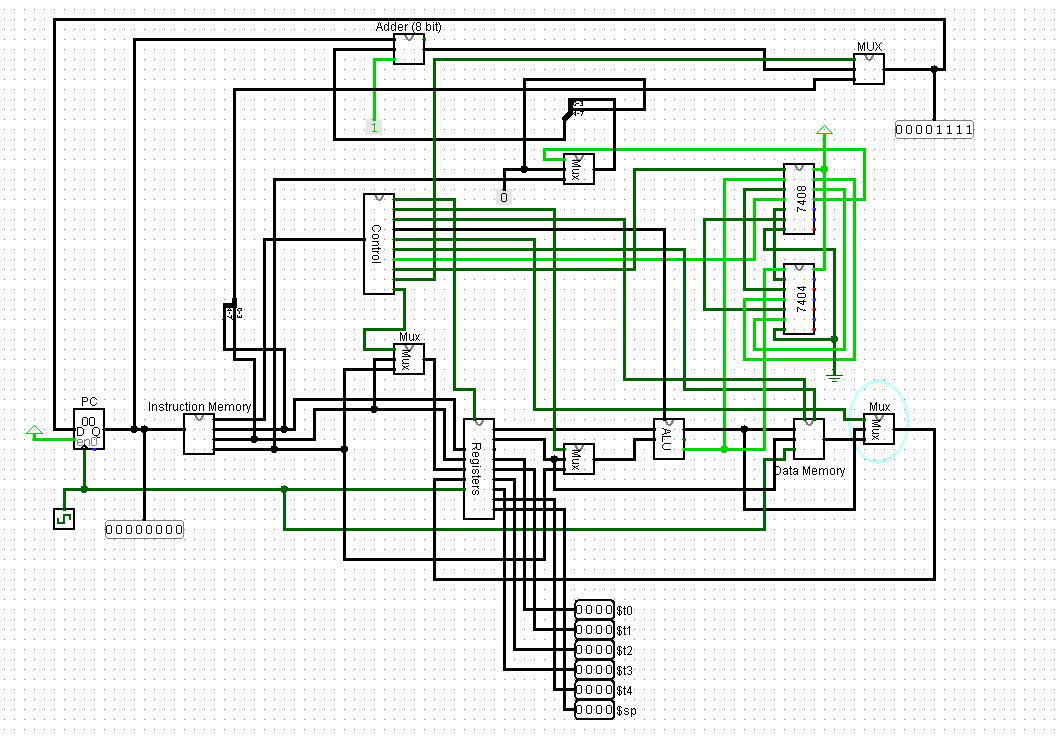
\includegraphics[height = 15 cm, width=1\linewidth]{completeBlockDiagram.png}
    \caption{4-bit MIPS Processor}
\end{figure}
\newpage
\section{Block diagrams of the main components}
\vspace{0.5cm}
\subsection{Instruction Memory with PC}
\vspace{0.5cm}
\begin{figure}[H]
    \centering
    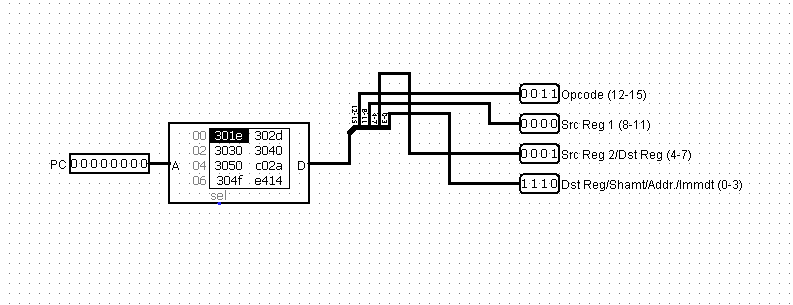
\includegraphics[width=1\linewidth]{insMemWPC.png}
    \caption{Instruction Memory with PC}
\end{figure}



\subsection{Data Memory with the Stack}
\vspace{0.5cm}
\begin{figure}[H]
    \centering
    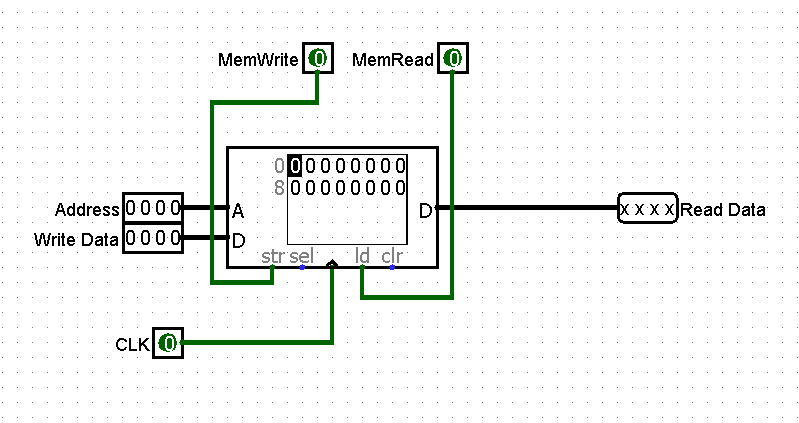
\includegraphics[width=1\linewidth]{dataMemWStack.png}
    \caption{Data Memory with the Stack} 
\end{figure}
\vspace{0.5cm}
\subsection{Register File}
\vspace{0.5cm}
\begin{figure}[H]
    \centering
    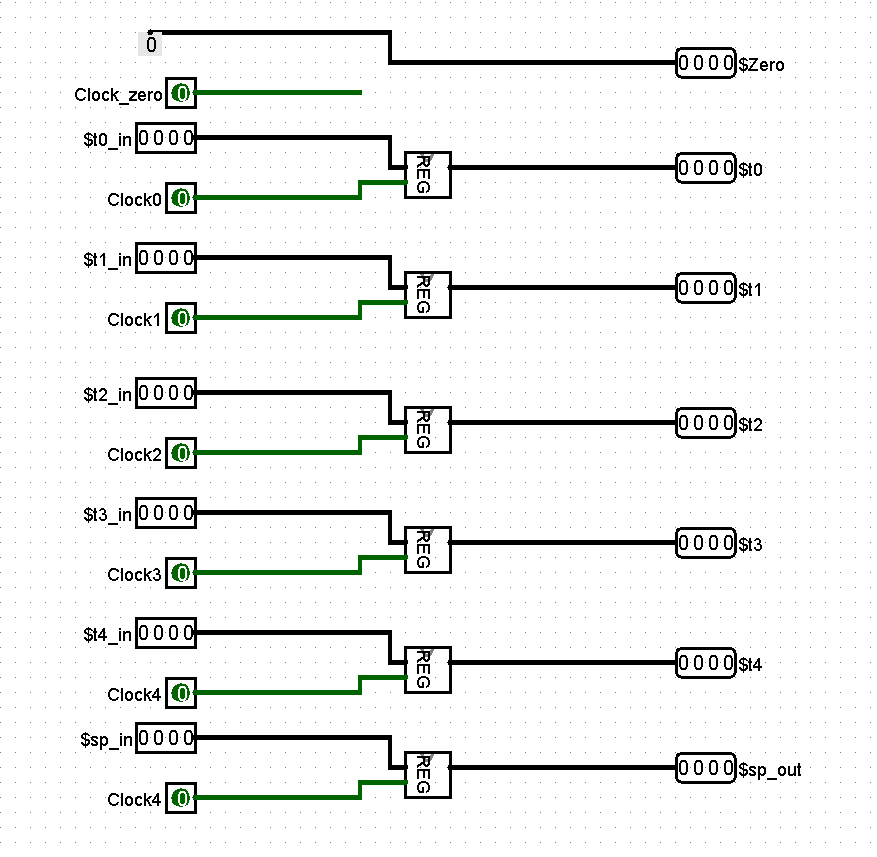
\includegraphics[height = 15 cm, width=1.2\linewidth]{registerFile.png}
    \caption{Register File} 
\end{figure}
\vspace{0.5cm}
\subsection{Control Unit}
\vspace{0.5cm}
\begin{figure}[H]
    \centering
    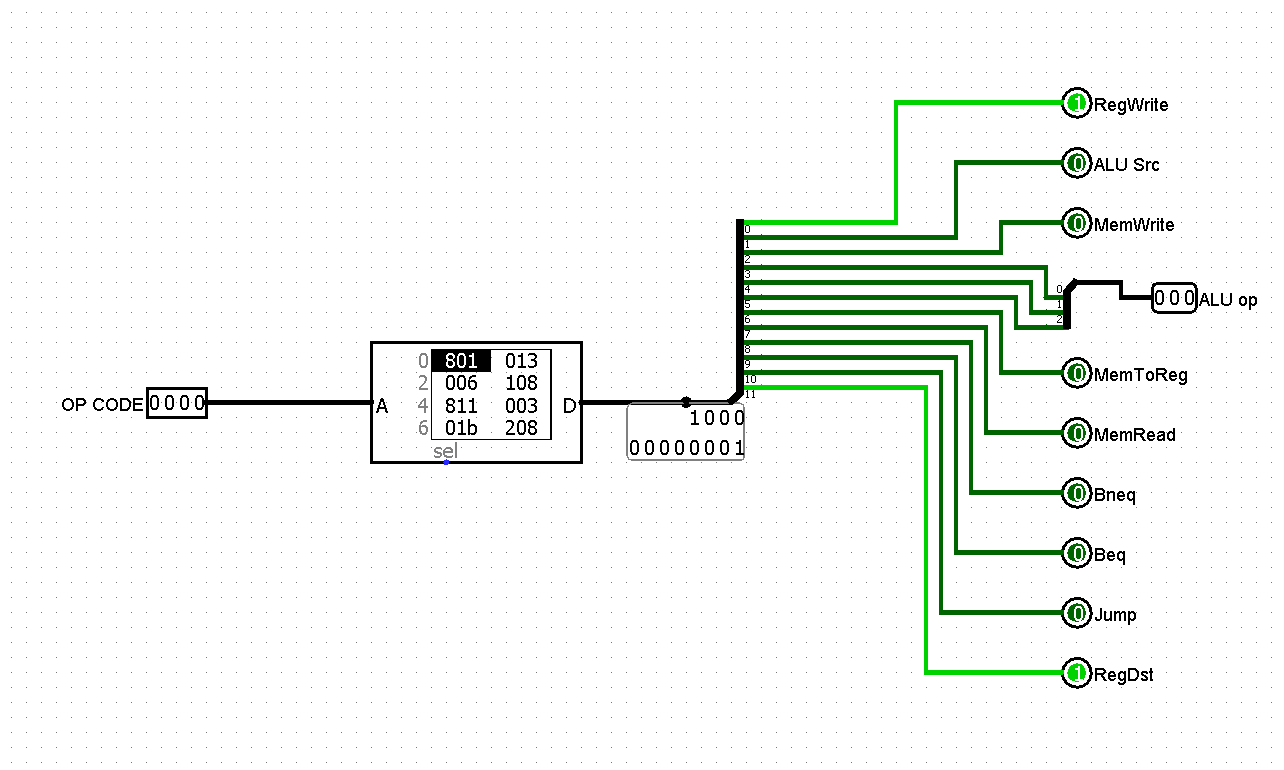
\includegraphics[width=1\linewidth]{controlUnit.png}
    \caption{Control Unit} 
\end{figure}

\section{Approach to implement the push and pop instructions}
\vspace{0.4cm}
We have implemented push and pop instructions using the assembler that we made using \textit{FLEX} and \textit{BISON}. We have made use of sw, lw, addi, subi operations here.
\newpage
\subsection{PUSH Operation}
\vspace{0.4cm}
The \textbf{push\_instruction} non-terminal in \texttt{parser.y} handles the implementation of PUSH.
\vspace{0.5cm}
\textbf{Implementation Steps:}\\
\textbf{Store Value:} The value to be pushed is typically stored in a register.\\
\textbf{Update Stack Pointer:} After storing the value, the stack pointer needs to be decremented to point to the next available memory location.\\

\textbf{PUSH REGISTER}\\
Example: PUSH \$t0\\
Explanation:
\begin{itemize}
    \item The machine code instructions generated for this PUSH operation involve storing the value of register \$t0 onto the stack and updating the stack pointer.
    \item Suppose the current stack pointer \$sp points to address 0x1000.
    \item The value of register \$t0 needs to be pushed onto the stack.
    \item Let's assume that \$t0 contains the value 0xABCD.
    \item The generated machine code instructions might look something like this:
    \begin{enumerate}
        \item \texttt{sw \$t0, 0(\$sp)} - Store the value of \$t0 (0xABCD) at memory address 0x1000.
        \item \texttt{subi \$sp, \$sp, 1} - Update the stack pointer to point to the next available memory location 0x0FFF, decrementing it by 1.
          \end{enumerate}
\end{itemize}
\vspace{0.35cm}
\textbf{PUSH INT LPAREN REGISTER RPAREN}\\
Example: PUSH 8(\$t1)\\
Explanation:
\begin{itemize}
    \item This form of PUSH operation involves loading a value from memory into a register and then pushing that value onto the stack.
    \item Let's assume that \$t1 contains the value 0x2000 and we want to push the value stored at memory address 0x2008 onto the stack.
    \item The generated machine code instructions might look like this:
    \begin{enumerate}
        \item \texttt{lw \$t1, 8(\$t1)} - Load the value stored at memory address 0x2008 into register \$t1.
      \item \texttt{sw \$t1, 0(\$sp)} - Store the value of \$t1 (value at 0x2008) onto the stack at the current stack pointer address.
      \item \texttt{subi \$sp, \$sp, 1} - Update the stack pointer to point to the next available memory location, decrementing it by 1.
      \end{enumerate}
      \end{itemize}
\subsection{POP Operation}
The \textbf{pop\_instruction} non-terminal handles the implementation of POP operation.\\
\textbf{POP REGISTER}\\
Example: `POP \$t2`\\
Explanation:
\begin{itemize}
    \item The machine code instructions generated for this POP operation involve loading a value from the stack into register \$t2 and updating the stack pointer.
    \item Suppose the current stack pointer \$sp points to address 0x0FFF.
    \item The value to be popped from the stack is stored at memory address 0x1000.
    \item The generated machine code instructions might look like this:
    \begin{enumerate}
        \item \texttt{lw \$t2, 0(\$sp)} - Load the value stored at memory address 0x1000 into register \$t2.
       \item \texttt{addi \$sp, \$sp, 1} - Update the stack pointer to point to the next available memory location 0x1000, incrementing it by 1.
    \end{enumerate}
\end{itemize}

In summary, PUSH and POP instructions manipulate the stack by storing and loading values using sw and lw operations respectively, and they update the stack pointer accordingly to reflect changes in the stack structure. These operations ensure proper stack management during program execution.\\

\section{ICs used with their count}
\begin{table}[H]
    \centering
    \begin{tabular}{|c|c|c|}
    \hline
        Name & IC Number & Count \\
    \hline
        40 pin microprocessor & ATmega32  & 6\\
        \hline
        4bit Binary Full Adder  & 7483 & 2\\
        \hline
        Quad 2 to 1 MUX & 74157 & 6\\
        \hline
    \end{tabular}
    \caption{ICs with counts}
\end{table}

\section{Simulator Info}
\textbf{Logisim} - Java Platform (Version 2.7.1)
\newpage
\section{Discussion}
\begin{itemize}
  \item We designed individual components in Logisim and recreated the whole circuit in Proteus to ease the hardware implementation.
  
  \item We learnt about probable incompatibility issues between HC and LS IC series. We avoided them during the hardware implementation.
  
  \item For the designing of ALU according to the given functions, we formed truth tables, used it to construct the required k-maps for $X_i$, $Y_i$ and $Z_i$, derived equations for each of them.

  \item We used 6 ATmega32 to separate the stages like a proper MIPS processor.
  \item For implementing the circuit in software level , we used 7400-library integrated circuits. In hardware level, necessary coding has been done at ATmega32 level.
  
\end{itemize}

\vspace{1cm}

\section{Contribution}
\begin{itemize}
    \item $2005034$ : Provided necessary codes and wrote the report taking help from everyone else. Lended a hand in hardware implementation. Helped in simulation in Proteus.
    
    \item $2005039$ : Managed all the hardware equipments, played a great role in hardware implementation. Simulated MIPS in Proteus.
    
    \item $2005042$ : Proposed the overall implementation idea and guided the team while designing the hardware. Designed the circuits in logisim and also contributed in Proteus simulation. Implemented MIPS processor in hardware.
    
    \item $2005043$ : Provided necessary help in report and codes. Helped in designing in Proteus.
    
    \item $2005059$ : Designed control unit, program counter, adder and MUX in logisim. Assisted in hardware implementation.
\end{itemize}


All of us collectively completed the 4-bits MIPS processor, going through multiple sessions of designing and debugging, lending each other shoulders. After 3-4 days of uncertainty, we finally saw our hardwork 


\end{document}
